% Implementation chart of the gradient-boosted comparator arm (R/09b_xgboost.R),
% in the format of the engine chart. Drawn 2026-09-25 from
% docs/figs/callgraph/boosters.md: the boxes from its reachable-function
% table, the arrows from its call edges and its table of targets. Redrawn the
% same day after the arrow check was added to the checker; every arrow here
% is backed by a row of those tables except the one `ex` arrow, which crosses
% the process boundary (the bundle written by the training run and read by
% the apply runners). `python docs/figs/callgraph_check.py boosters` holds
% this chart to the parser-based call graph. Engine boxes are referred to by
% number (E 3.9 is box 3.8 of pipeline_implementation.tex).
%
% Build:  pdflatex pipeline_boosters.tex   (from this directory)
\documentclass[10pt]{article}
\usepackage[paperwidth=44cm,paperheight=40cm,margin=8mm]{geometry}
\usepackage[T1]{fontenc}
\usepackage{lmodern}
\usepackage{amsmath}
\usepackage{tikz}
\usetikzlibrary{arrows.meta,fit,backgrounds,calc,positioning}
\pagestyle{empty}
\begin{document}
\centering
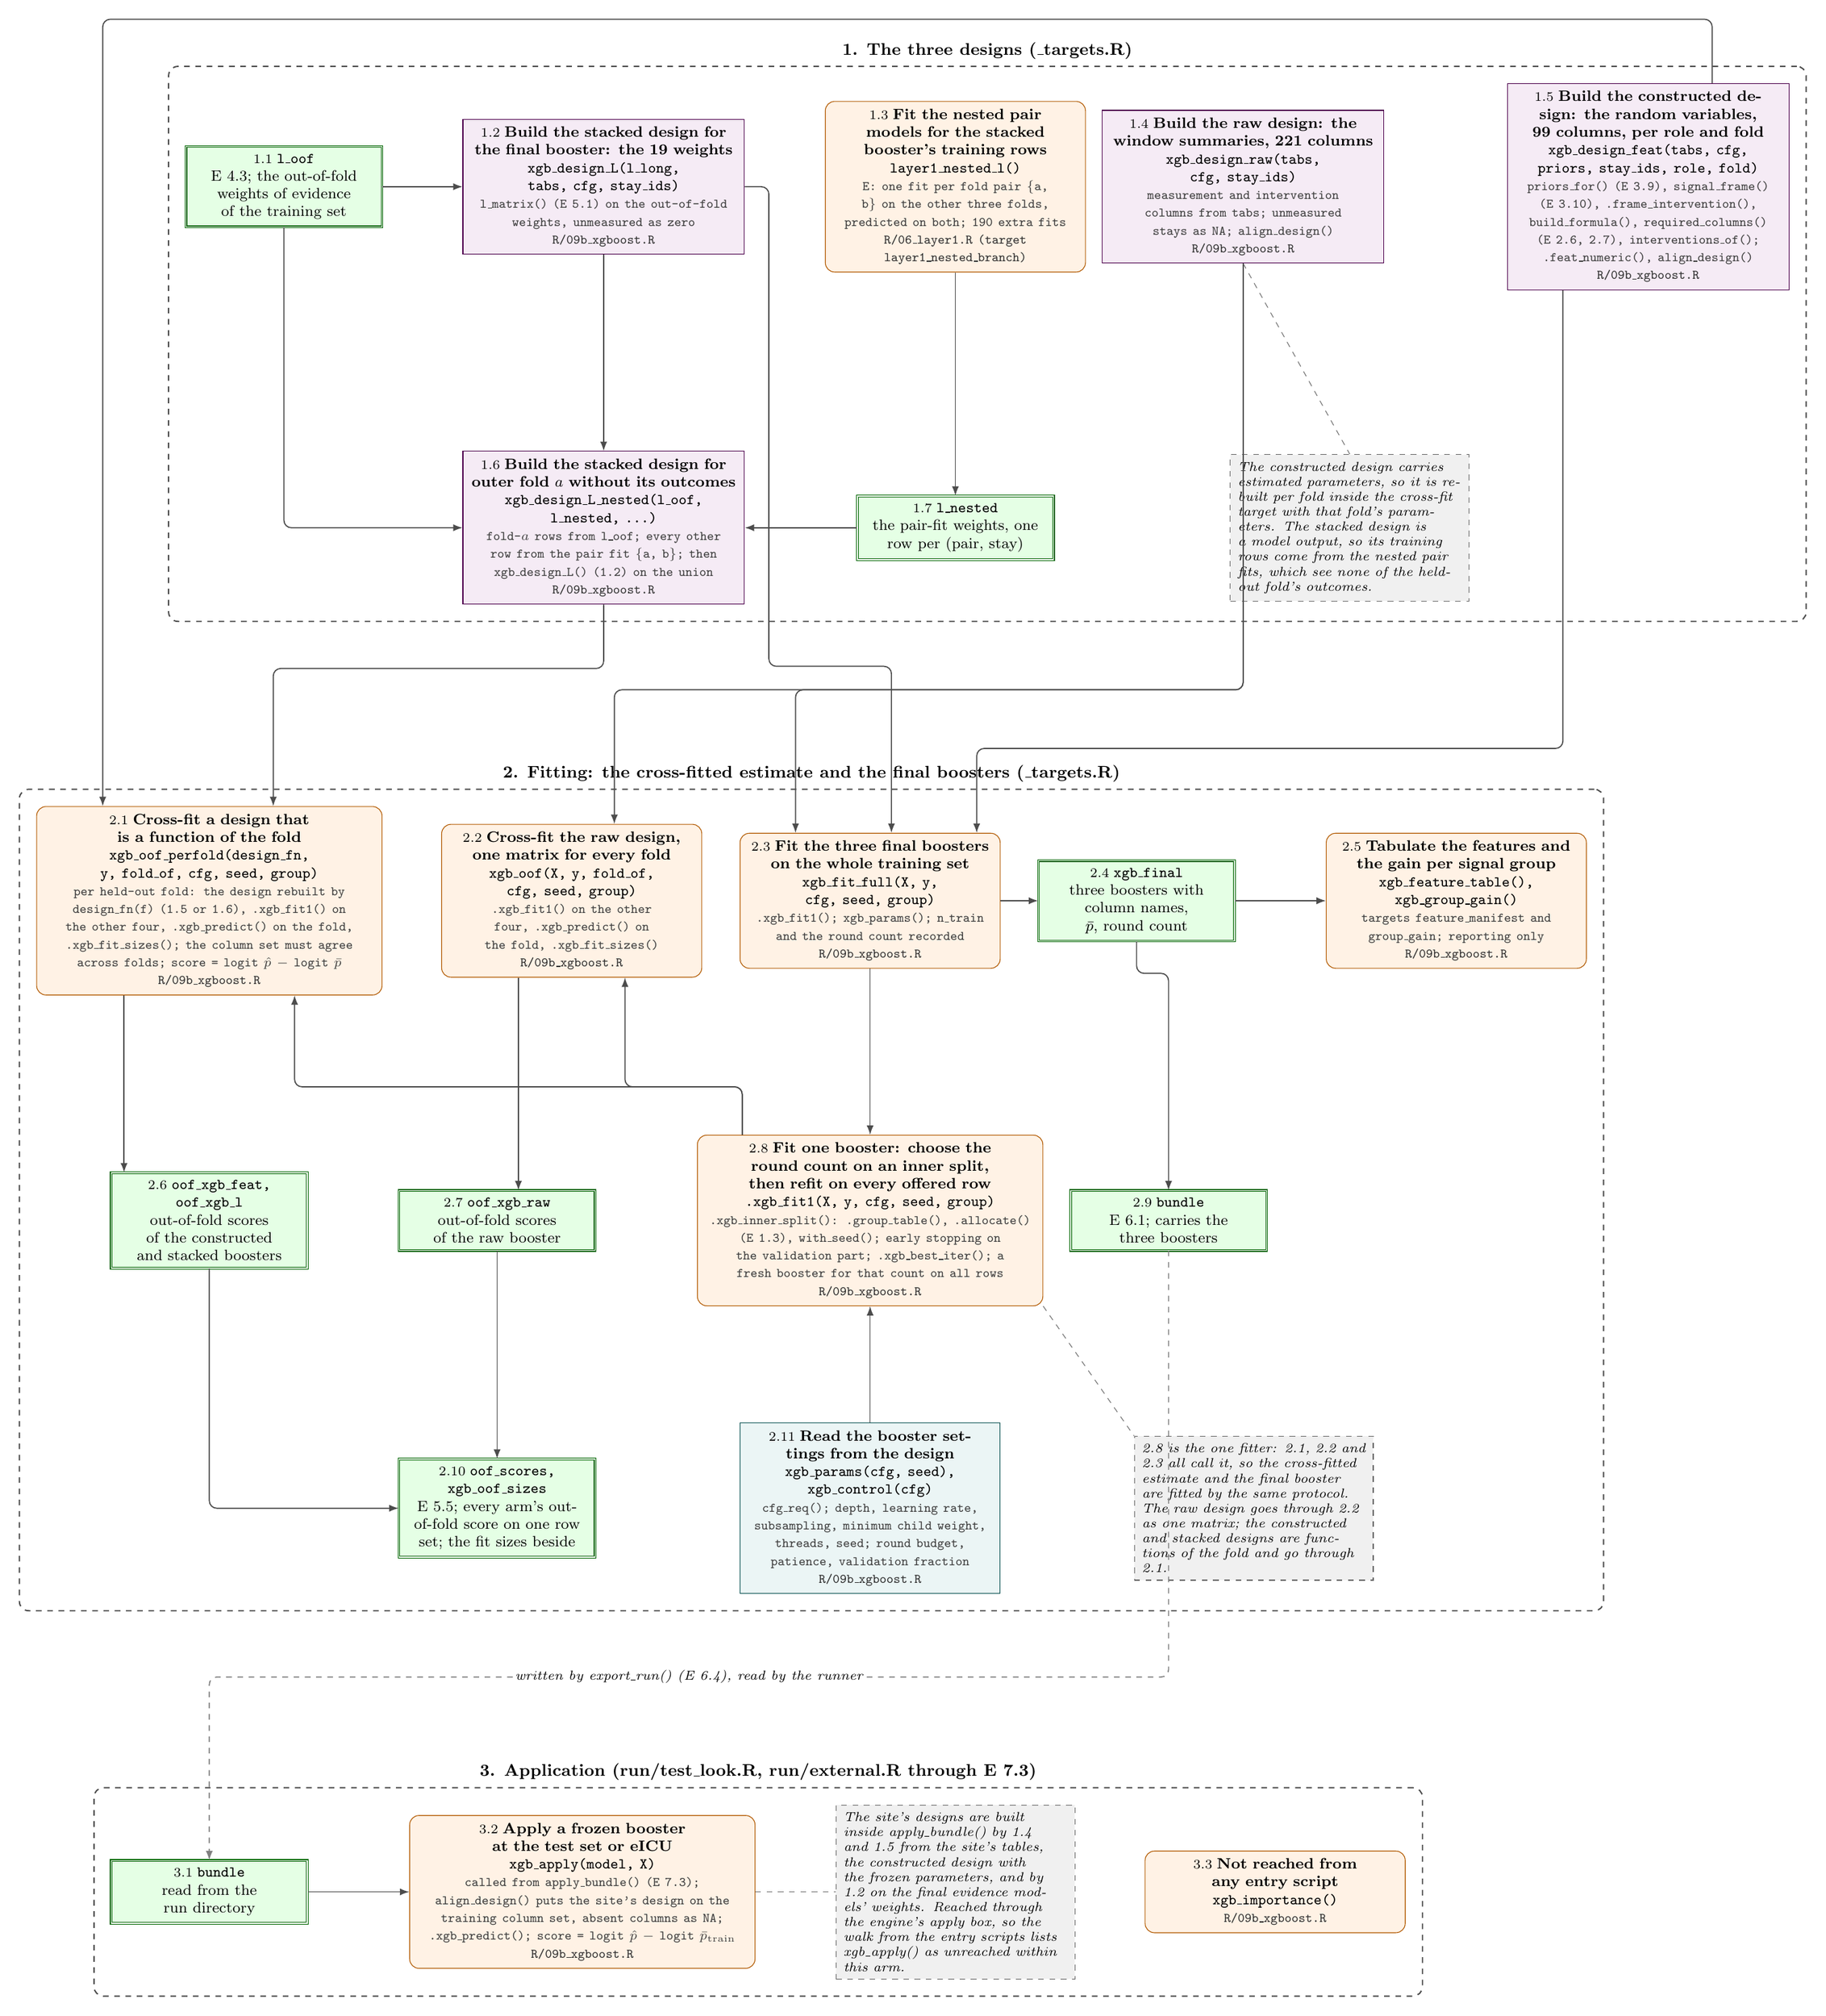
\begin{tikzpicture}[
  font=\footnotesize, x=1cm, y=1cm,
  fn/.style={draw=orange!70!black, fill=orange!10, rounded corners=5pt, align=center, inner sep=4pt, text width=4.6cm},
  fnw/.style={fn, text width=6.2cm},
  obj/.style={draw=blue!50!black!60, fill=blue!8, rounded corners=2pt, align=center, inner sep=4pt, text width=3.4cm},
  dcl/.style={draw=teal!60!black, fill=teal!8, align=center, inner sep=4pt, text width=4.6cm},
  dsg/.style={draw=violet!60!black, fill=violet!8, align=center, inner sep=4pt, text width=5.0cm},
  outp/.style={draw=green!40!black, fill=green!10, double, align=center, inner sep=4pt, text width=3.4cm},
  note/.style={draw=black!60, dashed, fill=black!6, align=left, inner sep=4pt, text width=4.2cm, font=\scriptsize\itshape},
  e/.style={-{Latex[length=5pt]}, line width=0.6pt, draw=black!70, rounded corners=4pt},
  ex/.style={e, dashed, draw=black!50},
  en/.style={draw=black!55, dashed, line width=0.4pt},
  grp/.style={draw=black!70, dashed, line width=0.7pt, inner sep=9pt, rounded corners=5pt},
  lab/.style={font=\small\bfseries, anchor=south},
  al/.style={font=\scriptsize\itshape, fill=white, inner sep=1pt}]

\newcommand{\B}[5]{{\scriptsize #1}\;\textbf{#2}\\\texttt{\textbf{#3}}\\{\scriptsize\ttfamily\color{black!75}#4}\\{\scriptsize\ttfamily\color{black!80}#5}}
\newcommand{\Bs}[4]{{\scriptsize #1}\;\textbf{#2}\\\texttt{\textbf{#3}}\\{\scriptsize\ttfamily\color{black!80}#4}}
\newcommand{\Obj}[3]{{\scriptsize #1}\;\texttt{\textbf{#2}}\\#3}

% =====================================================================
% STAGE 1: the three designs and what feeds them
% =====================================================================
\node[outp] (loof) at (5.0,0) {\Obj{1.1}{l\_oof}{E 4.3; the out-of-fold weights of evidence of the training set}};
\node[dsg] (dL) at (11.0,0) {\B{1.2}{Build the stacked design for the final booster: the 19 weights}{xgb\_design\_L(l\_long, tabs, cfg, stay\_ids)}{l\_matrix() (E 5.1) on the out-of-fold weights, unmeasured as zero}{R/09b\_xgboost.R}};
\node[fn] (nested) at (17.6,0) {\B{1.3}{Fit the nested pair models for the stacked booster's training rows}{layer1\_nested\_l()}{E: one fit per fold pair \{a, b\} on the other three folds, predicted on both; 190 extra fits}{R/06\_layer1.R (target layer1\_nested\_branch)}};
\node[dsg] (raw) at (23.0,0) {\B{1.4}{Build the raw design: the window summaries, 221 columns}{xgb\_design\_raw(tabs, cfg, stay\_ids)}{measurement and intervention columns from tabs; unmeasured stays as NA; align\_design()}{R/09b\_xgboost.R}};
\node[dsg] (feat) at (30.6,0) {\B{1.5}{Build the constructed design: the random variables, 99 columns, per role and fold}{xgb\_design\_feat(tabs, cfg, priors, stay\_ids, role, fold)}{priors\_for() (E 3.9), signal\_frame() (E 3.10), .frame\_intervention(), build\_formula(), required\_columns() (E 2.6, 2.7), interventions\_of(); .feat\_numeric(), align\_design()}{R/09b\_xgboost.R}};

\node[dsg] (dLn) at (11.0,-6.4) {\B{1.6}{Build the stacked design for outer fold $a$ without its outcomes}{xgb\_design\_L\_nested(l\_oof, l\_nested, ...)}{fold-$a$ rows from l\_oof; every other row from the pair fit \{a, b\}; then xgb\_design\_L() (1.2) on the union}{R/09b\_xgboost.R}};
\node[outp] (lnested) at (17.6,-6.4) {\Obj{1.7}{l\_nested}{the pair-fit weights, one row per (pair, stay)}};
\node[note] (n1) at (25.0,-6.4) {The constructed design carries estimated parameters, so it is rebuilt per fold inside the cross-fit target with that fold's parameters. The stacked design is a model output, so its training rows come from the nested pair fits, which see none of the held-out fold's outcomes.};

\draw[e] (loof) -- (dL);
\draw[e] (loof.south) |- (dLn.west);
\draw[e] (dL) -- (dLn);
\draw[e] (nested) -- (lnested);
\draw[e] (lnested) -- (dLn);
\draw[en] (raw.south) -- (n1.north);

\begin{scope}[on background layer]
\node[grp, fit=(loof)(dL)(nested)(raw)(feat)(dLn)(lnested)(n1), label={[lab]north:{1. The three designs (\_targets.R)}}] (b1) {};
\end{scope}

% =====================================================================
% STAGE 2: fitting: the cross-fitted estimate and the final boosters
% =====================================================================
\node[fnw] (perfold) at (3.6,-13.4) {\B{2.1}{Cross-fit a design that is a function of the fold}{xgb\_oof\_perfold(design\_fn, y, fold\_of, cfg, seed, group)}{per held-out fold: the design rebuilt by design\_fn(f) (1.5 or 1.6), .xgb\_fit1() on the other four, .xgb\_predict() on the fold, .xgb\_fit\_sizes(); the column set must agree across folds; score = logit $\hat p$ $-$ logit $\bar p$}{R/09b\_xgboost.R}};
\node[fn] (oof) at (10.4,-13.4) {\B{2.2}{Cross-fit the raw design, one matrix for every fold}{xgb\_oof(X, y, fold\_of, cfg, seed, group)}{.xgb\_fit1() on the other four, .xgb\_predict() on the fold, .xgb\_fit\_sizes()}{R/09b\_xgboost.R}};
\node[fn] (full) at (16.0,-13.4) {\B{2.3}{Fit the three final boosters on the whole training set}{xgb\_fit\_full(X, y, cfg, seed, group)}{.xgb\_fit1(); xgb\_params(); n\_train and the round count recorded}{R/09b\_xgboost.R}};
\node[outp] (finalobj) at (21.0,-13.4) {\Obj{2.4}{xgb\_final}{three boosters with column names, $\bar p$, round count}};
\node[fn] (ftbox) at (27.0,-13.4) {\B{2.5}{Tabulate the features and the gain per signal group}{xgb\_feature\_table(), xgb\_group\_gain()}{targets feature\_manifest and group\_gain; reporting only}{R/09b\_xgboost.R}};

\node[outp] (featobj) at (3.6,-19.4) {\Obj{2.6}{oof\_xgb\_feat, oof\_xgb\_l}{out-of-fold scores of the constructed and stacked boosters}};
\node[outp] (rawobj) at (9.0,-19.4) {\Obj{2.7}{oof\_xgb\_raw}{out-of-fold scores of the raw booster}};
\node[fnw] (fit1) at (16.0,-19.4) {\B{2.8}{Fit one booster: choose the round count on an inner split, then refit on every offered row}{.xgb\_fit1(X, y, cfg, seed, group)}{.xgb\_inner\_split(): .group\_table(), .allocate() (E 1.3), with\_seed(); early stopping on the validation part; .xgb\_best\_iter(); a fresh booster for that count on all rows}{R/09b\_xgboost.R}};
\node[outp] (bundleobj) at (21.6,-19.4) {\Obj{2.9}{bundle}{E 6.1; carries the three boosters}};

\node[outp] (scoresobj) at (9.0,-24.8) {\Obj{2.10}{oof\_scores, xgb\_oof\_sizes}{E 5.5; every arm's out-of-fold score on one row set; the fit sizes beside}};
\node[dcl] (par) at (16.0,-24.8) {\B{2.11}{Read the booster settings from the design}{xgb\_params(cfg, seed), xgb\_control(cfg)}{cfg\_req(); depth, learning rate, subsampling, minimum child weight, threads, seed; round budget, patience, validation fraction}{R/09b\_xgboost.R}};
\node[note] (n2) at (23.2,-24.8) {2.8 is the one fitter: 2.1, 2.2 and 2.3 all call it, so the cross-fitted estimate and the final booster are fitted by the same protocol. The raw design goes through 2.2 as one matrix; the constructed and stacked designs are functions of the fold and go through 2.1.};

% designs -> consumers
\draw[e] (dLn.south) -- ++(0,-1.2) -| ($(perfold.north)+(1.2,0)$);
\draw[e] ($(feat.north)+(1.2,0)$) -- ++(0,1.2) -| ($(perfold.north)+(-2.0,0)$);
\draw[e] (raw.south) -- ++(0,-8.0) -| ($(oof.north)+(0.8,0)$);
\draw[e] (raw.south) -- ++(0,-8.0) -| ($(full.north)+(-1.4,0)$);
\draw[e] ($(feat.south)+(-1.6,0)$) -- ++(0,-8.6) -| ($(full.north)+(2.0,0)$);
\draw[e] (dL.east) -- (14.1,0) -- (14.1,-9.0) -- (16.4,-9.0) -- ($(full.north)+(0.4,0)$);
% the one fitter
\draw[e] (full) -- (fit1);
\draw[e] ($(fit1.north)+(-2.4,0)$) -- ++(0,0.9) -| ($(oof.south)+(1.0,0)$);
\draw[e] ($(fit1.north)+(-2.4,0)$) -- ++(0,0.9) -| ($(perfold.south)+(1.6,0)$);
\draw[e] (par) -- (fit1);
% outputs
\draw[e] ($(perfold.south)+(-1.6,0)$) -- ($(featobj.north)+(-1.6,0)$);
\draw[e] ($(oof.south)+(-1.0,0)$) -- ($(rawobj.north)+(0.4,0)$);
\draw[e] (full) -- (finalobj);
\draw[e] (finalobj) -- (ftbox);
\draw[e] (finalobj.south) -- ++(0,-0.6) -| (bundleobj.north);
\draw[e] (rawobj) -- (scoresobj);
\draw[e] (featobj.south) |- (scoresobj.west);
\draw[en] (fit1.south east) -- (n2.north west);

\begin{scope}[on background layer]
\node[grp, fit=(perfold)(oof)(full)(finalobj)(ftbox)(featobj)(rawobj)(fit1)(bundleobj)(scoresobj)(par)(n2), label={[lab]north:{2. Fitting: the cross-fitted estimate and the final boosters (\_targets.R)}}] (b2) {};
\end{scope}

% =====================================================================
% STAGE 3: application
% =====================================================================
\node[outp] (bundleapp) at (3.6,-32.0) {\Obj{3.1}{bundle}{read from the run directory}};
\node[fnw] (apply) at (10.6,-32.0) {\B{3.2}{Apply a frozen booster at the test set or eICU}{xgb\_apply(model, X)}{called from apply\_bundle() (E 7.3); align\_design() puts the site's design on the training column set, absent columns as NA; .xgb\_predict(); score = logit $\hat p$ $-$ logit $\bar p_{\mathrm{train}}$}{R/09b\_xgboost.R}};
\node[note] (n3) at (17.6,-32.0) {The site's designs are built inside apply\_bundle() by 1.4 and 1.5 from the site's tables, the constructed design with the frozen parameters, and by 1.2 on the final evidence models' weights. Reached through the engine's apply box, so the walk from the entry scripts lists xgb\_apply() as unreached within this arm.};
\node[fn] (imp) at (23.6,-32.0) {\Bs{3.3}{Not reached from any entry script}{xgb\_importance()}{R/09b\_xgboost.R}};

\draw[ex] (bundleobj.south) -- ++(0,-8.0) -| (bundleapp.north) node[al, pos=0.25] {written by export\_run() (E 6.4), read by the runner};
\draw[e] (bundleapp) -- (apply);
\draw[en] (apply) -- (n3);

\begin{scope}[on background layer]
\node[grp, fit=(bundleapp)(apply)(n3)(imp), label={[lab]north:{3. Application (run/test\_look.R, run/external.R through E 7.3)}}] (b3) {};
\end{scope}
\end{tikzpicture}
\end{document}
